% Gemini theme
% See: https://rev.cs.uchicago.edu/k4rtik/gemini-uccs
% A fork of https://github.com/anishathalye/gemini

\documentclass[final]{beamer}

% ====================
% Packages
% ====================
\usepackage{pgf}  

\usepackage[T1]{fontenc}
\renewcommand{\seriesdefault}{bx}
\usepackage{lmodern}
\usepackage[size=custom,width=96,height=48,scale=1.5]{beamerposter}
\usetheme{gemini}
\usecolortheme{uchicago}
\usepackage{graphicx}
\usepackage{booktabs}
\usepackage{tikz}
\usepackage{pgfplots}
\pgfplotsset{compat=1.17}
\usepackage[superscript,biblabel]{cite}
% ====================
% Lengths
% ====================

% If you have N columns, choose \sepwidth and \colwidth such that
% (N+1)*\sepwidth + N*\colwidth = \paperwidth
\newlength{\sepwidth}
\newlength{\colwidth}
\setlength{\sepwidth}{0.025\paperwidth}
\setlength{\colwidth}{0.3\paperwidth}
\newlength{\sepwid}
\newlength{\onecolwid}
\newlength{\twocolwid}
\newlength{\threecolwid}
\setlength{\paperwidth}{53.33in} % A0 width: 46.8in
\setlength{\paperheight}{40in} % A0 height: 33.1in
\setlength{\sepwid}{0.02\paperwidth} % Separation width (white space) between columns
\setlength{\onecolwid}{0.25\paperwidth} % Width of one column
\setlength{\twocolwid}{0.44\paperwidth} % Width of two columns
\setlength{\threecolwid}{0.708\paperwidth} % Width of three col

\newcommand{\separatorcolumn}{\begin{column}{\sepwid}\end{column}}

% ====================
% Title
% ====================

\title{Determinants of Economic Growth: A Reinforcement Learning Approach}

\author{Savin Khadka \and Munisamy Gopinath}
\institute{}
\author{Savin Khadka \inst{1} \and Munisamy Gopinath \inst{1}}

\institute[shortinst]{\inst{1} Dept of Ag. and Applied Economics, University of Georgia}


% ====================
% Footer (optional)
% ====================

\footercontent{
  \hfill AAEA Annual Meeting 2021, Austin TX \hfill
  \href{mailto:srkhadka@uga.edu}{srkhadka@uga.edu}}
% (can be left out to remove footer)

% ====================
% Logo (optional)
% ====================

% use this to include logos on the left and/or right side of the header:
% \logoright{
\includegraphics{logos/CAES-FS-FC.eps}}
% \logoleft{
\includegraphics{logos/uga.eps}}
% ====================
% Body
% ====================
\begin{document}


\begin{frame}[t]
\begin{columns}[t]
\separatorcolumn

\begin{column}{\onecolwid}

\begin{block}{Introduction}

What drives economic growth and why do differentials in growth exist across nations?  Theoretical examinations of these questions have been unable to provide a comprehensive explanation so far, and they often differ on the relative importance of variables such as technological advancement, human capital accumulation, trade openness, and quality of institutions in the growth of an economy. Empirical studies, on the other hand, face a significant problem of model uncertainty, because selection of the proper empirical model is limited by theory, leading to more than 140 variables being proposed as determinants of growth in the literature.\cite{moral2012determinants} We explore a novel data-driven approach to solving the economic growth puzzle by extending a Reinforcement Learning (RL) multi-agent simulation framework\cite{zheng2020ai} to identify the key determinants of economic growth.
\end{block}


\begin{alertblock}{Objectives}
\begin{itemize}
    \item \textbf{To investigate the role of proposed growth determinants in driving economic growth}
    
    \item \textbf{To examine the sensitivity of growth trajectory to initial conditions}
\end{itemize}
\end{alertblock}

\begin{block}{Methods}
\begin{itemize}
    \item A 2-D environment is configured with resource endowments (stone and wood) and geographic constraints (water bodies) wherein agents may gather and trade resources. 
    \item Agents have the ability to use one each of their collected resources to build a house upon which they will receive a reward. The value of reward from building is determined by the agent's skill parameter.  
    \item Multiple simulation episodes are conducted under varying environmental parameters including agents' skill distribution, resource-generation properties, trade restrictions, and central planning. 
    \item Welfare of agents under different initial conditions and policies are compared across episodes.
\end{itemize}
\vspace{0.8cm}
\centering 
\includegraphics[scale = 1.4]{logos/uga.eps}
\end{block}
\end{column}


\begin{column}{\twocolwid}
\begin{figure}
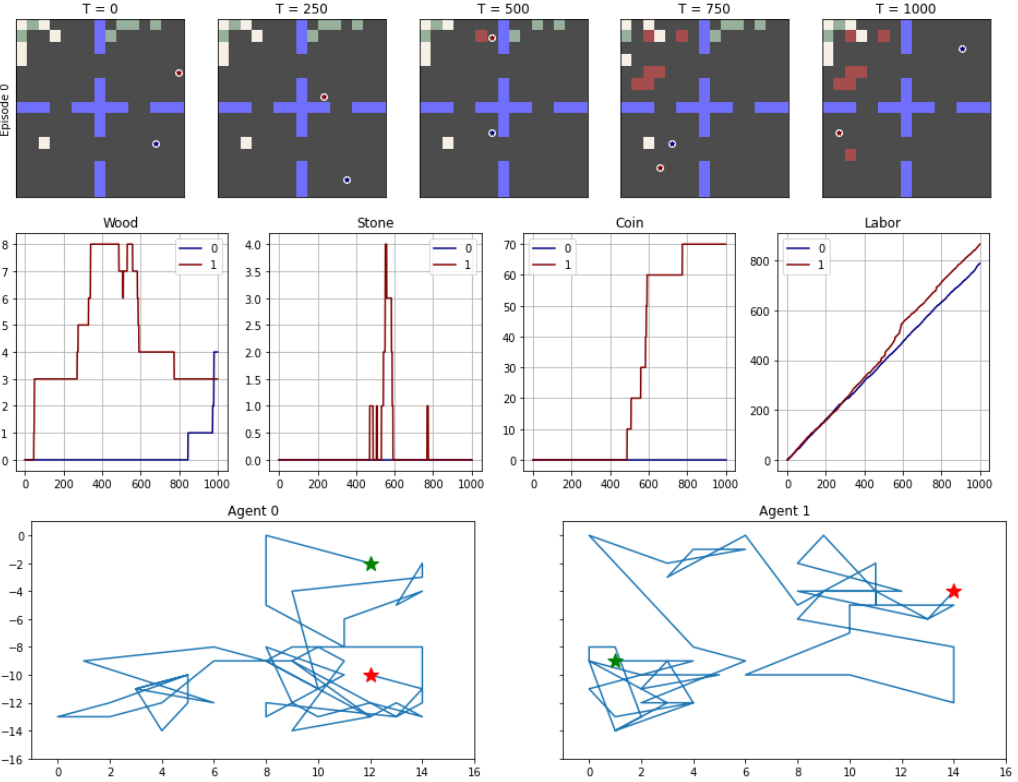
\includegraphics[height = 32.5cm]{figs/quadrant-notrading.png}
\caption{Two-agent quadrant world with no trading}
\end{figure}
\begin{figure}
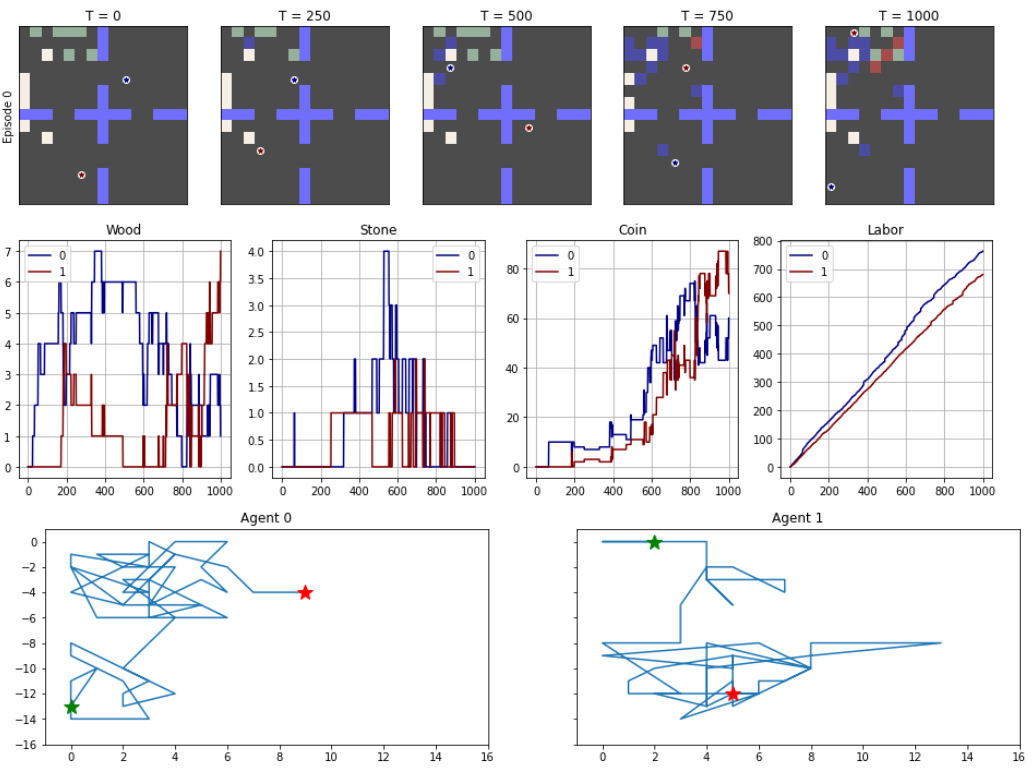
\includegraphics[height = 32.5cm]{figs/quadrant-trading2.png}
\caption{Two-agent quadrant world where agents are allowed to trade}
\end{figure}

\begin{block}
\small{In the figures above, the first row shows the state of the world at multiple periods during the course of a simulation episode. The second row shows resources acquired and labor supplied by the agents, and the third row traces  their paths across the world (red = initial position).}
\end{block}


\end{column}




\begin{column}{\onecolwid}
\begin{block}{Agent Behavior}
Agents share a utility function that is concave and increasing in money ($x^c_{i,t}$) and linearly decreasing in labor ($l_{i,t}$)\cite{zheng2020ai}:
\begin{equation}
   u_i(x_{i,t}, l_{i,t}) =  \text{CRRA}(x^c_{i,t}) - l_{i,t}, \hspace{.5cm} 
\end{equation}
Each agent optimizes their total discounted utility over time \cite{zheng2020ai} by solving:
\begin{equation}
    \begin{aligned}
       \underset{\pi_i}{\text{max}} \quad \mathbb{E}_{a_i \sim \pi_i, \textbf{a}_{-i} \sim \textbf{\pi}_{-i}, s^{'} \sim \tau}  \left[ \sum_{t=1}^H \lambda^t \times r_{i,t}+ u_i(x_{i,0}, l_{i,0})\right], \\ \text{where} \quad
       r_{i,t} \equiv  u_i(x_{i,t}, l_{i,t}) - u_i(x_{i,t-1}, l_{i, t-1})) 
    \end{aligned}
\end{equation}
\end{block}


\begin{block}{Preliminary Results}
    \begin{itemize}
        \item Agent welfare is extremely sensitive to initial conditions. This can be seen in Figure 1 where Agent 1 (shown in red) starts with better access to randomly-generated resources that are represented by white and gray blocks along the top margin. Consequently, at the end of the simulation episode, Agent 1 is able to acquire significantly more coins than Agent 0. 
        
        \item Asymmetry in agent welfare decreases when agents are allowed to trade among themselves. Figure 2 shows results from a simulation where agents can trade resources via a continuous double auction (submitting bids and asks to a market). 
    \end{itemize}
  \end{block}

  \begin{block}{Potential Extensions}
  \begin{itemize}
      \item \textbf{Human capital accumulation}: allow agents to buy skill-increasing widgets in exchange for resources 
      \item \textbf{Alliance}: allow proximate agents to form groups among themselves to further collective interests
      \item \textbf{Recreating historical episodes}: attempt to recreate historical growth experiences (e.g., East Asian, Chilean) by fine-tuning environment parameters 
  \end{itemize}
  \vspace{0.25cm}
  \end{block}


\begin{block}{References}
\small{\bibliographystyle{plain}
\bibliography{poster}}
\end{block}

\end{column}

\separatorcolumn
\end{columns}
\end{frame}

\end{document}
